\onehalfspacing

\section{Lösungsansatz}

Bei der prototypischen Lösung steht im Zentrum dieser Arbeit die Wissensdatenbank \textit{Wikidata}\footnote{URL: \url{https://www.wikidata.org/wiki/Wikidata:Main_Page} (letzter Zugriff am 20.05.2022).} als offener Forschungsdatenmanagement-Service. Bei Wikidata handelt sich ursprünglich um ein offenes dankenbankbasiertes Angebot von Wikimedia für strukturierte Daten im Wiki*versum, das das Konzept von Linked Open Data umsetzt. Damit ist es flexibel und sprachenunabhängig einsetzbar, wodurch es als Modell auch für Forschungsdatenmanagement in der akademischen Wissenschaft interessant wird. Tatsächlich wird dieser Weg im Rahmen von NFDI gegenwärtig bestritten. Das \textit{Open Science Lab} am ,,Leibniz-Informationszentrum Technik und Naturwissenschaften und Universitätsbibliothek''\footnote{URL: \url{https://www.tib.eu/de/} (letzer Zugriff am 20.05.2022).} hat für das Konsortium \textit{NFDI4Culture}\footnote{URL: \url{https://nfdi4culture.de/index.html} (letzter Zugriff am 20.05.2022).} Wikidata und insbesondere die zugrunde liegende Software \textit{Wikibase}\footnote{URL: \url{https://wikibase.consulting/what-is-wikibase/} (letzter Zugriff am 20.05.2022).} auf die Einsetzbarkeit für ein Forschungsdatenmanagement von Kulturdaten hin evaluiert. Erste Ergebnisse wurden im März 2022 auf dem TIB-Blog veröffentlicht.\footnote{Siehe Lozana Rossenova (2022): Examining Wikidata and Wikibase in the context of research data management applications, veröffentlicht am 16.03.2022 auf dem TIB-Blog, URL: \url{https://blogs.tib.eu/wp/tib/2022/03/16/examining-wikidata-and-wikibase-in-the-context-of-research-data-management-applications/}.} Parallel führt das NFDI4Culture-Konsortium selbst die Workshop-Reihe ,,Wikibase'' durch.\footnote{URI: \url{https://nfdi4culture.de/resource/E2261/about.html}.} 

Auch im Kontext historischer Forschung kommt Wikidata bereits zum Einsatz. Das Online-Portal ,,Archivführer. Deutsche Kolonialgeschichte'' nutzt Wikidata als zentralen Datenspeicher für strukturierte Daten, die in Zusammenhang mit dem Thema ,,Deutsche Kolonien und Schutzgebiete'' stehen.\footnote{Das Projekt wurde 2017 an der Fachhochschule Potsdam initiiert und ist vom Auswärtigen Amt gefördert worden, URL: \url{https://archivfuehrer-kolonialzeit.de/} (letzter Zugriff am 20.05.2022).} Das Portal führt lediglich die Wikidata-Daten für die Datenpräsentation zusammen und ermöglicht einen multiperpektivischen Zugang zu den Daten.\footnote{Zum Beispiel Georeferenzierung der Orte anhand historischen Kartenmaterials, URL: \url{https://archivfuehrer-kolonialzeit.de/map} (letzter Zugriff am 20.05.2022).} Die Besonderheit ist, dass die Datenbereitstellung durch Wikidata ermöglicht, über die Projektlaufzeit hinaus Daten von jeder/jedem erweitern zu lassen sowie diese in gänzlich anderen Kontexten zu verwenden. Darüber hinaus verfolgt das Projekt das Ziel, die Daten mit der ,,kolonialen Vergangenheiten anderer Ländern''\footnote{URL: \url{https://archivfuehrer-kolonialzeit.de/about} (letzter Zugriff am 20.05.2022).} zu verknüpfen und auf diese Weise das Forschungsfeld zum Deutschen Kolonialismus anschlussfähig an die Forschung zum Europäischen Kolonialismus zu machen. Die Zusammenarbeit und der kollaborative Austausch dazu erfolgen ebenfalls global in Wikidata mit dem ,,Wikidata:WikiProject European Colonialism''.\footnote{URL: \url{Wikidata:WikiProject European Colonialism} (letzter Zugriff am 20.05.2022).} Das internationale Projekt ,,European Holocaust Research Infrastructure'' (EHRI), welches im Rahmen der Open Science-Strategie von der Europäischen Kommission seit 2017 gefördert wird\footnote{Im EU-Programm ,,Horizon Europe'', das bis 2027 läuft, URL: \url{https://ec.europa.eu/info/research-and-innovation/funding/funding-opportunities/funding-programmes-and-open-calls/horizon-europe_en}. Projektwebsite von EHRI, URL: \url{https://www.ehri-project.eu/} (alle letzter Zugriff am 20.05.2022).} nutzt Wikidata als zentrales Verzeichnis zur Erstellung einer Liste von Ghettos aus der Zeit des Holocausts.\footnote{Nancy Cooey (2018): Using Wikidata to build an authority list of Holocaust-era ghettos, veröffentlicht am 12.02.2018 auf dem EHRI Document Blog, URL: \url{https://blog.ehri-project.eu/2018/02/12/using-wikidata/\#Selecting\_Wikidata\_as\_a\_Tool} (letzter Zugriff am 20.05.2022).} Ziel ist, Daten aus verschiedenen Enzyklopädien, die bisher isoliert waren, in Wikidata erstmals zusammenzuführen und zu verknüpfen.\footnote{Vgl. ebd. Zentrale Enzyklopädien sind ,,The Yad Vashem Encyclopedia of the Ghettos During the Holocaust'' von Yad Vashem (Israel) und ,,USHMM Encyclopedia of Camps and Ghettos'' des United States Holocaust Memorial Museum (USA).}

Grundsätzlich ist bei der Implementierung des offenen Forschungsdatenmanagements mit Wikidata ist zu beachten, dass hier das Konzept von Linked (Open) Data umgesetzt wird, bei dem es sich, wie in Kapitel 2.2.2 bereits erläutert wurde, um einen wesentlichen Baustein des \textit{Semantic Web} handelt. Damit erfolgt offenes FDM in der höchsten Open Data-Stufe (= 5 Sterne). Vorteil ist, dass auf diese Weise Stärken dieses Konzepts, welche vor allem in der Verknüpfung und Vernetzung von Daten liegen, für das Forschungsdatenmanagement ausgenutzt werden können. Nachteilig ist, dass dieser Ansatz voraussetzungsreicher als andere Lösungen ist, da zum einen Kenntnisse der allgemeinen Technologien von Linked Data Web wie RDF (Resource Description Framework), JSON-LD (JavaScript Object Notation for Linked Data) oder URI (Uniform Ressource Identifier)\footnote{Im Rahmen dieser Arbeit können diese Technologien nicht detailliert vorgestellt werden, daher wird auf Grundlagenliteratur verwiesen. Siehe zum Beispiel Christian Stein: Linked Open Data – Wie das Web zur Semantik kam, in: Bibliothek Forschung und Praxis (Hrsg.), Band 38, Nr. 3, 2014, S. 447-455, doi:10.1515/bfp-2014-0055; Patrick Danowski, Adrian Pohl: (Open) Linked Data in Bibliotheken, Berlin, Boston, 2013, doi:10.1515/9783110278736; Gradmann, Steffen Hennicke, Marlies Olensky: Linked Data, in: Digitale Dienste für die Wissenschaft (Hrsg.), 2012, S. 18-22, doi.org/10.18452/6627;  } und zum anderen Kenntnisse des spezifische Metadatenschemas bzw. der Onotologie zugrunde liegenden Software Wikibase von Wikidata.\footnote{Siehe Mediawiki (2022): Wikibase/DataModel, URL:\url{https://www.mediawiki.org/wiki/Wikibase/DataModel} (letzter Zugriff am 22.05.2022).} für die Umsetzung benötigt werden.

\section{Erhebung}

\begin{quote}
    [...] Dass dieses methodisches Vorgehen auch transparent und nachvollziehbar ist.\footnote{B4\_Transkript, Pos. 67.}
\end{quote}

Datenerhebung in der empirischen historischen Forschung geht mit historischer Quellenanalyse und Quellenkritik einher.\footnote{Vgl. W. H. Schröder: Historische Sozialforschung: Forschungsstrategie - Infrastruktur - Auswahlbibliographie.
Historical Social Research, in: Supplement (Hrsg.) 1988, Nr. 1, S. 1-109, hier S. 15ff., URN: \url{https://nbn-resolving.org/urn:nbn:de:0168-ssoar-286038}
} Anders als in der naturwissenschaftlichen Datenerhebung, wo anhand von Experimenten, Beobachtungen, Simulationen oder Messungen, Daten in Echtzeit gewonnen werden und dementsprechend die Erhebungsmethoden an den Forschungsfragen angepasst werden können, ist die Vorgehensweise bei den geschichtswissenschaftlichen Disziplinen maßgeblich von der Überlieferungstruktur und der Quellensituation abhängig.\footnote{Was zu einem ,,Quellenproblem'' führen kann, siehe dazu ebd. S. 19f.} Informationen zum Entstehungskontext sowie zur Erhebungsmethode sind also essentiell, um Forschungsdaten im Sinne einer Datenkritik kontextualisieren, verstehen und damit letztlich bewerten zu können. Bei den Forschungsdaten zu jüdischen Gewerbebetrieben sind diese jedoch nicht hinterlegt und es handelt sich daher bisher um implizites Wissen, was eine Nachnutzung erschwert oder sogar unmöglich machen kann. Hinsichtlich der Nachvollziehbarkeit und Transparenz von Forschungsdaten ist daher Ziel von offenem Forschungsdatenmanagement, das Wissen um den Entstehungskontext sowie um die geschichtswissenschaftliche Datenerhebungsmethode explizit zu machen. 

\subsection{Entstehungskontext}

Im Forschungsfeld ist der Großteil der Forschungsdaten zu jüdischen Gewerbebetrieben in lokalen wissenschaftlichen Forschungsprojekten erhoben worden. Hinsichtlich des Entstehungskontextes sind also zwei Informationen relevant: erstens die Forschungsprojekte selbst und zweitens die projektzugehörigen Personen. In Wikidata werden sie als eigene \textit{Items} angelegt.\footnote{Ausführlich zum Konzept der Wikidata-Items siehe URL: \url{https://www.wikidata.org/wiki/Help:Items} (letzter Zugriff am 21.05.2022).} Dadurch erhalten sie einen Identifikator nach dem Schema \textit{Q} und können eindeutig den zugehörigen Forschungsdaten zugeordnet werden. In Wikidata erfolgt die Modellierung nach dem Linked Data-Prinzip auf Basis des Datenmodells der zugrunde liegenden Wikibase-Software. Im Rahmen dieser Arbeit kann dieses Modell nicht im Detail 


Die Frage, wie die verschiedenen (akademischen) Forschungsaktivitäten zur semantische Anreicherung von Forschungsdaten konzeptionalisiert und formalisiert werden können, scheint gegenwärtig noch nicht Gegenstand des Forschungsdatenmanagements zu sein, denn einen wissenschaftlichen Standard, nach denen diese beschrieben werden können und sollen, konnte nicht gefunden werden. Zwar gibt es generische Metadatenstandards wie \textit{Dublin Core} der \textit{Dublin Core Metadata Initiative}\footnote{URL: \url{https://www.dublincore.org/specifications/dublin-core/dcmi-terms/} (letzter Zugriff am 15.05.2022)} oder \textit{DataCite}\footnote{URL: \url{https://datacite.org/} (letzter Zugriff am 15.05.2022)} des gleichnamigen internationalen Konsortiums. Aber deren Schemata enthalten kein Konzept ,,Forschungvorhaben'' oder ,,Forschungsprojekt''. Lediglich das DataCite-Schema enthält dazu vereinzelt Elemente ,,Funding Reference'' , die aber optional sind.


Daher können keine allgemeingültigen Aussagen darüber gemacht werden, welche Informationen im Rahmen des Enstehungskontexts im Sinne guter wissenschaftlicher Praxis benötigt werden. Deutlich geworden ist, dass die Forschungsdaten zu jüdischen Gewerbebetrieben mehrheitlich in lokalen Forschungsprojekten erhoben wurden. Detaillierte Informationen sind jedoch unklar.


um Allerdings stellen vereinzelte Einrichtungen zentrale Verzeichnisse, mit denen sie ihre Forschungsprojekte verzeichnen. standardisiert erfasst und eindeutig identifizierbar sind, gibt es nicht. Die Deutsche Forschungsgemeinschaft (DFG) hat immerhin mit dem Informationssystem ,,GEPRIS – Geförderte Projekte der DFG'' (GEPRIS)\footnote{URL: \url{https://gepris.dfg.de/gepris/OCTOPUS?task=showAbout} (letzter Zugriff am 21.05.2022).} in Auszügen ihre Daten zu allen gegenwärtigen und vergangenen geförderten Projekten veröffentlicht. Dort ist zum Beispiel auch das Forschungsprojekt ,,Geschichte mittlerer und kleiner jüdischer Unternehmen in Frankfurt am Main und Breslau 1929/39 bis 1945'' verzeichnet mit Informationen über Antragssteller, Fachliche Zuordnung, Förderzeitraum, Projektkennung, Projektergebnissen und -beschreibung. 

nicht groß diskutieren sondern einfach machen




Zweitens, kann mittels eines eindeutigen Identifikators auf das Froschungsprojekt referenziert werden. Dieser Ansatz setzt bereits vorhandene Verzeichnisse voraus, welche . Auf die Forschungsdaten aus dem Berliner Projekt bezogen, müsste also das zugehörige . Eine standardisierte und zentrale Projektverzeichnung gibt es dort jedoch (noch) nicht.\footnote{} Zudem müsste sichergestellt sein, dass abgelaufene Projekte archiviert werden.

 


\begin{figure}[h]
    \centering
    \frame{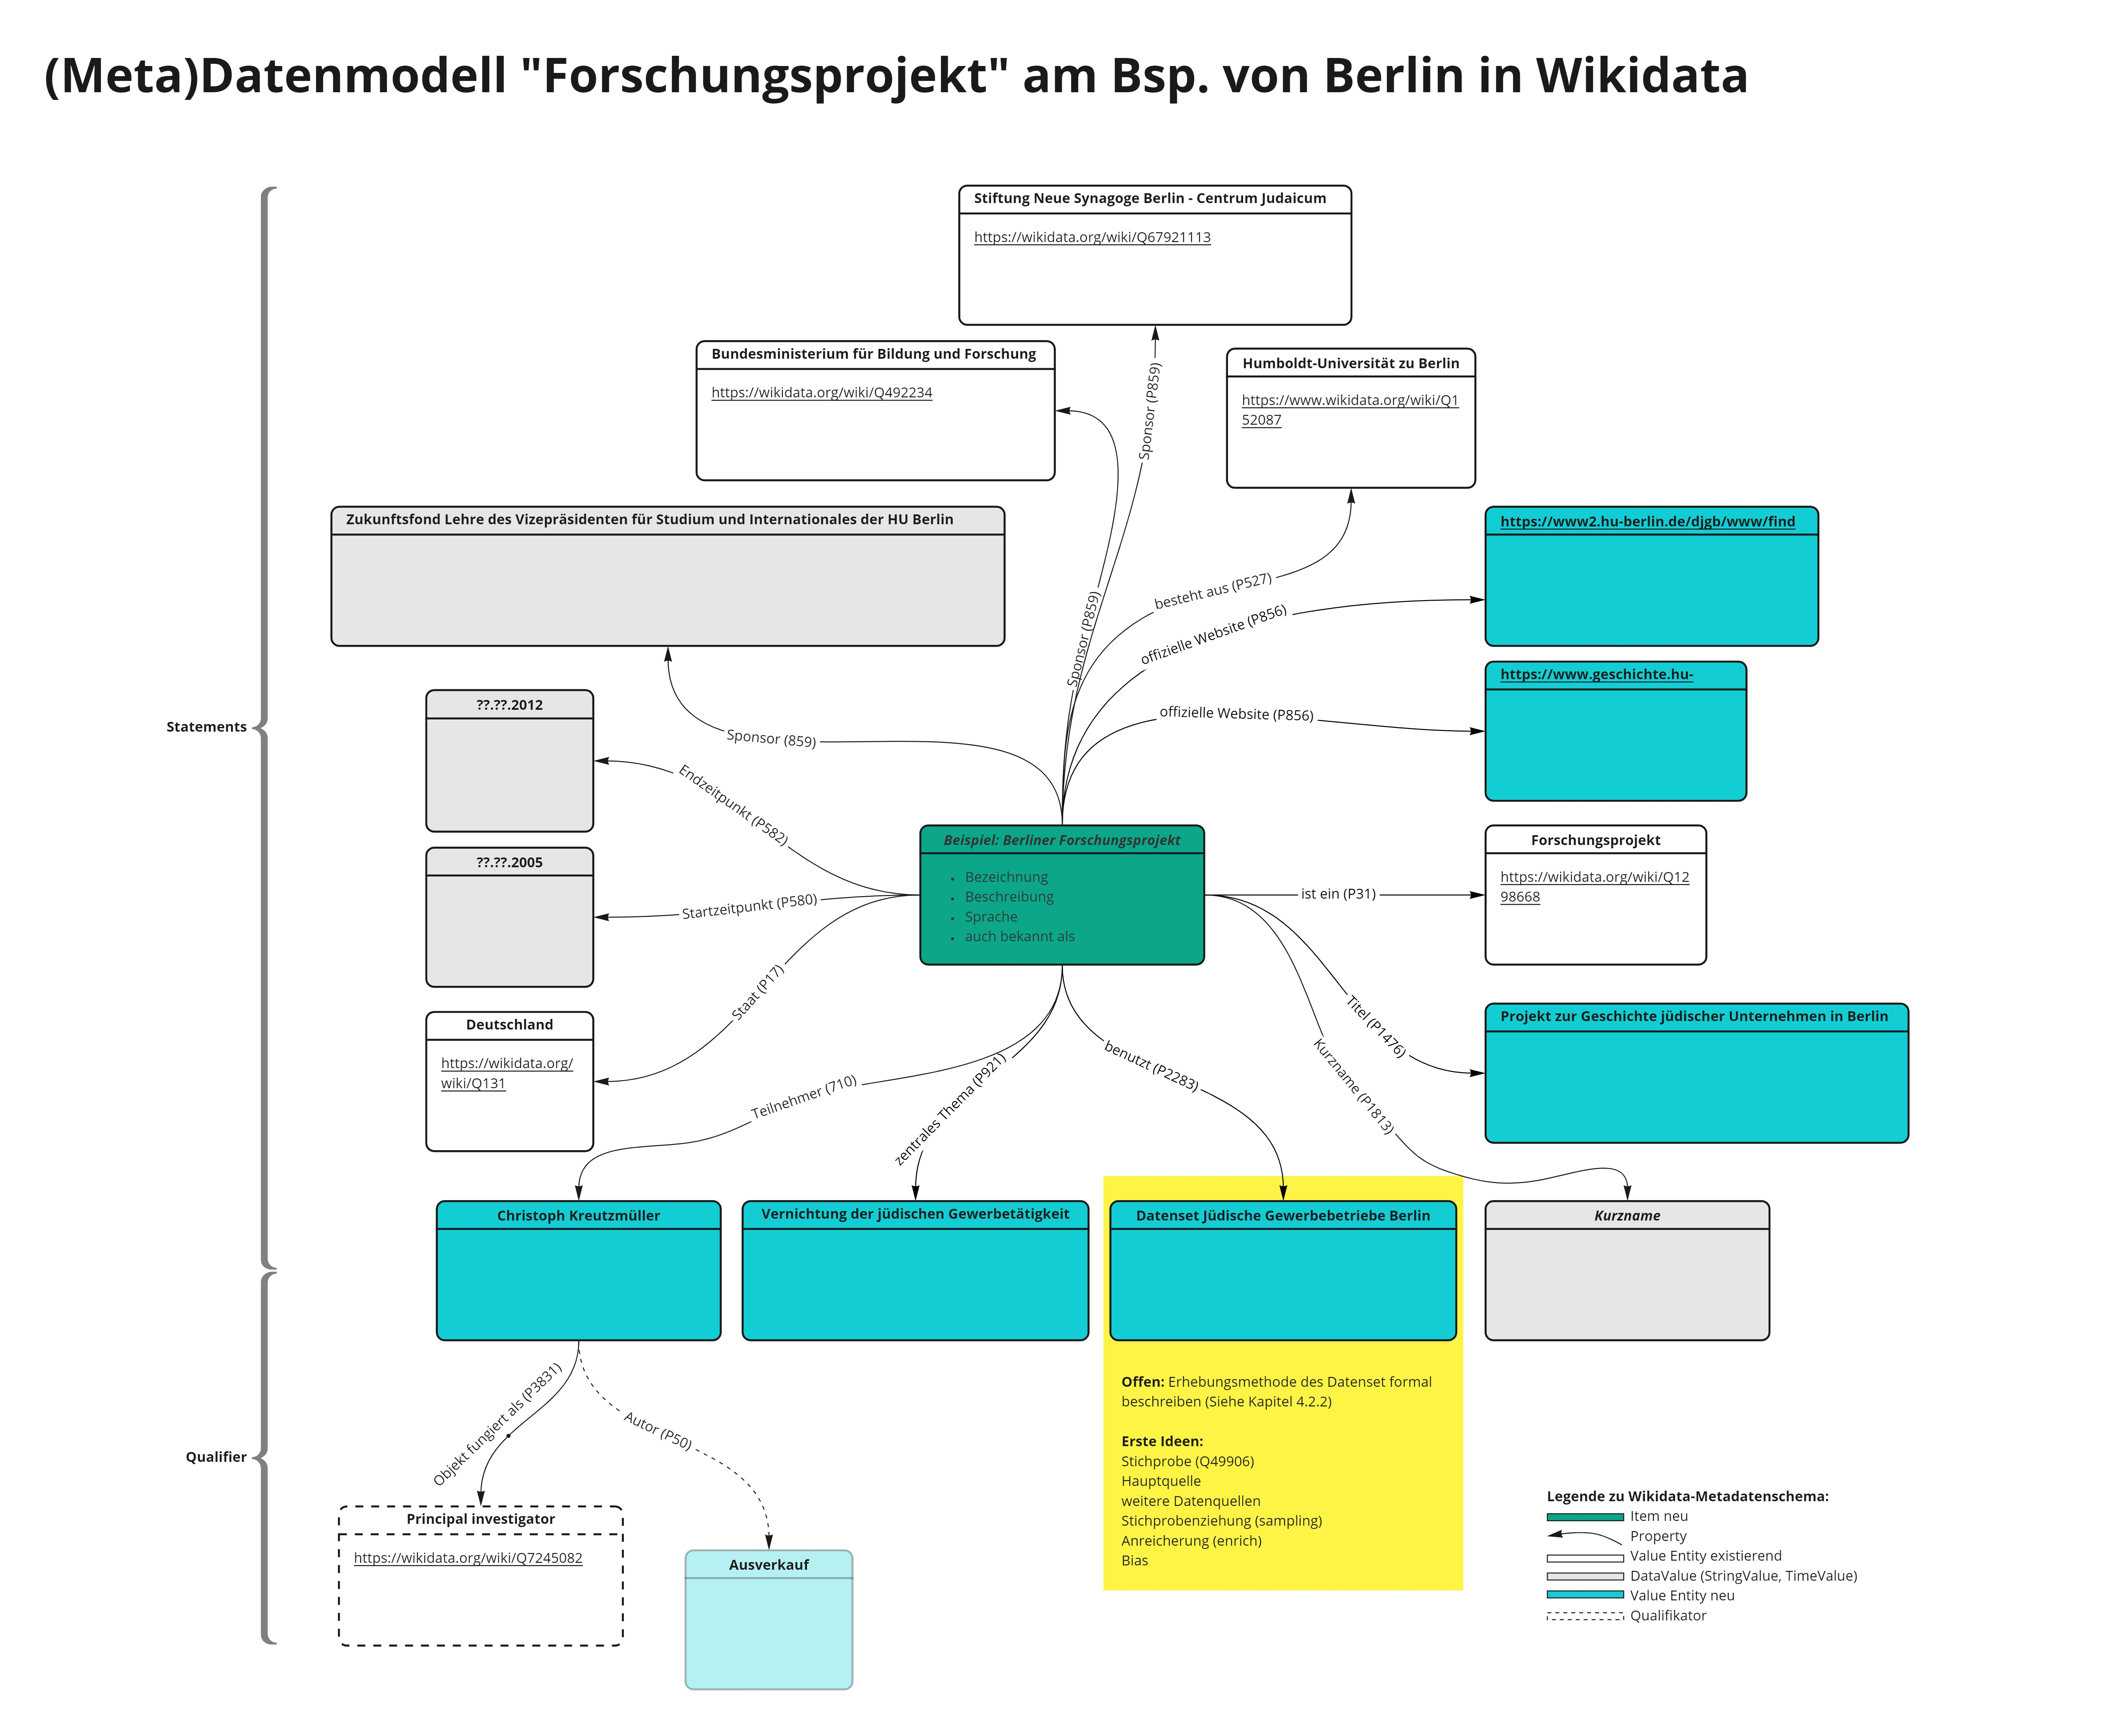
\includegraphics[scale=0.3]{wikidata-item_research-project}}
    \caption{Modellierung der lokalen Forschungsprojekte in Wikidata.\protect\footnotemark}
    \label{fig:x cubed graph}
\end{figure}








 

\footnote{Diese Informationen konnten anhand der Publikation extrahiert werden, siehe Kreutzmüller 2012, S. 7-13.}



aber sind, lassen sich aus diesen Information extrahieren. Damit stellt sich abre immer noch die Frage, wie Forschungsprojekte -vorhaben beschrieben werden könne.
Es geht folglich um die formale Erschließung der Forschungsdaten. Diese Erschließung erfolgt anhand von Metadaten, die die inhaltserschließenden Daten beschreiben (Daten über Daten). 
Zu der Frage also wie Forschungsprojekte oder -vorhaben konzeptionalisert, formalisiert und spezifisiert werden können, scheint derzeit noch gar nicht Gegenstand von Forschungsdatenmanagement zu sein. Semantische Metadaten Schwerpunkt liegt


Das Forschungsdatenmanagement an der Humboldt-Universität zu Berlin empfiehlt bezüglich des Entstehungskontextes entweder eine schriftliche Dokumentation in Form einer Readme-Datei oder die Verwendung von strukturierten Metadaten unter Heranziehung von fachübergreifenden Metadatenstandards wie zum Beispiel .\footnote{HU Berlin (2022): Dokumentation und Metadaten, URL: \url{https://www.cms.hu-berlin.de/de/dl/dataman/teilen/dokumentation/metadaten} (letzter Zugriff am 21.05.2022).}, die Auffindbarkeit und Interoperabilität gewährleisten. Da Wikidata vorwiegend strukturierte Daten hat, können rein textuelle Dokumentationen ausgeschlossenen werden. 





Um , sind hier Metadatenstandards notwendig.\footnote{Vgl. forschungsdaten.info (2022): Metadaten und Metadatenstandards, URL: \url{https://www.forschungsdaten.info/themen/beschreiben-und-dokumentieren/metadaten-und-metadatenstandards/} (letzter Zugriff am 21.05.2022).} 
Es braucht einerseits also deskriptive Metadaten, die die Entstehung der Forschungsdaten beschreiben, und andererseits bibliografische Metadaten, die Forschungsdaten den historischen Quellen eindeutig zuordnen.







. Einen Standard zu formalen Beschreibung von Forschungsprojekten oder -vorhaben gibt es nicht  





\subsection{Erhebungsmethode}



Es braucht zum einen Informationen zum spezifischen Entstehungskontext der Daten (Datenherkunft). 

Aufgenommen werden daher strukturierte Informationen zur Datenherkunft, da diese essentiell sind bei der eindeutigen Zuordnung der Daten zu den einzelnen Forschungsprojekten, vor allem wenn das Forschungsdatenmanagement projektübergreifend ist und außerdem an andere Forschungsfelder andockt. An Standards orientieren, versuchen zu mappen


Auswertung der historischen Quellen (Datenerhebung)
historische Grundgesamtheit Teilmenge
Für die Nachvollziehbarkeit werden zum anderen Informationen zur Vorgehensweise der Datenerhebung, also zum methodischen Vorgehen, benötigt. Dafür existieren keine disziplinübergreifenden Metadatenstandards.\footnote{Vgl. forschungsdaten.info, URL: \url{https://www.forschungsdaten.info/themen/beschreiben-und-dokumentieren/metadaten-und-metadatenstandards/} (letzter Zugriff am 15.05.2022).} Das heißt, diese Metadaten sind fachspezifisch. Im naturwissenschaftlichen Bereich und in der Archäologie gibt es mit der \textit{Research Resource Identification Initiative} (RRI)\footnote{} und mit \textit{IANUS}\footnote{URL: \url{https://ianus-fdz.de/}. Der Support war nach Auslaufen der DFG-Projektförderung 2017 allerdings eingeschränkt. So konnten neue Datensammlungen bis 2022 nicht aufgenommen werden, siehe URL: \url{http://datenportal.ianus-fdz.de/pages/information.jsp\#dateneigentuemer} (alle letzter Zugriff 15.05.2022).} bereits zentrale Ansätze, wie Enstehungskontexte und Methodiken anhand von Thesauri oder festen Vokabularen formal beschrieben werden können.\footnote{Siehe zum Beispiel die Thesauri des Deutschen Archäologischen Instituts, URL: \url{http://thesauri.dainst.org/de.html} mit der Kollektion zu den Methoden, URL: \url{http://thesauri.dainst.org/de/collections/\_203bcc05.html} (alle letzter Zugriff am 15.05.2022).} Allerdings sind sie nicht übertragbar auf den geschichtswissenschaftlichen Bereich. Offenes Forschungsdatenmanagement ist hier mit zwei Herausforderungen konfrontiert. Erstens existiert ein fachspezifischer Standard für die Geschichtswissenschaften noch nicht. Zweitens ist fraglich, inwiefern sich die Forschungsdesigns im Forschungsfeld formalisieren lassen. Als essentiell wurden drei Informationen herausgearbeitet: Datenquellen, Erhebungsmethode, Bias. Die Datenquellen lassen sich wie folgt strukturieren:

\begin{enumerate}
    \item Datenquelle: Gedruckte Verzeichnisse und Listen sowie Karteisammlungen, in denen Gewerbebetriebe dezidiert als jüdisch markiert und veröffentlicht wurden\footnote{In München übernahm diese Aufgabe das städtische Gewerbeamt, vgl. Rappl 2000, S. 145f. In Frankfurt am Main war der zentrale Akteur die Industrie- und Handelskammer.} Sie enthalten die wesentlichen Grunddaten der Gewerbebetriebe wie Name, Inhaber, Branche und Adresse.
    \item Datenquelle: Verschiedene zeitgenössische Aktenbestände, die den Vorgang der Verfolgung einzelner Gewerbebetriebe verwaltungsseitig dokumentieren. 
    \item Datenquelle: Eine wichtige Quelle im Forschungsfeld stellen die Wiedergutmachungsakten, insbesondere der Rückerstattungsverfahren, nach 1945 dar, welche seit den 90er Jahren der historischen Forschung zugänglich sind und oft eine Ersatzüberlieferung für die vernichteten und zerstörten zeitgenössischen Quellen darstellen. Der Nachteil is     
\end{enumerate}

Zu den ersten beiden Datenquellen ist generell festzustellen, dass die Überlieferung als disparat und lückenhaft bezeichnet wurde, da viele Bestände teilweise oder überwiegend von den Nationaloszialisten vernichtet wurden, um Spuren zu verwischen, oder in den letzten Kriegstagen unwiederbringlich zerstört wurden. Oft sind nur Überreste und Splitter erhalten, was die Datenerhebung der Studien maßgeblich beeinflusste. Hierbei lassen sich zwei wesentliche Vorgehensweisen unterscheiden:

\begin{enumerate}
    \item Erhebungsmethode: Datenquelle 1 ist überliefert und bildet den Ausgangspunkt, mit der ein Sample von jüdischen Gewerbebetrieben zusammengestellt wurde. Dieses Sample mit den Grunddaten wurde anschließend mit den Datenquellen 2 und 3 abgeglichen und um Daten angereichert, die signifikante Veränderungen des Betriebs zeigten.  
    \item Erhebungsmethode: Datenquelle 1 ist nicht überliefert, weshalb alternative Wege für eine Stichprobenziehung gefunden werden mussten. In Hamburg kamen in erster Linie die Wiedergutmachungsakten sowie Bestände der Devisenstelle zum Einsatz.\footnote{Vgl. Bajohr 1998, S. 21ff.} In Berlin hat man ein gänzlich anderen Ansatz verfolgt. Dort wurden ein Sample anhand der Zentralhandelsregisterbeilage (ZHRB), welche dem Deutschen Reichsanzeiger und Preußischen Staatsanzeiger täglich beilag, erstellt und bis 1945 alle Firmenveränderungen aufgenommen. Damit wurde die ZHRB zwischen 1930 und 1939 einmal komplett digitalisiert. Erst danach wurden nacheinander die Gewerbebetriebe mit überlieferten Quellen und anderen Hinweisen abgeglichen und bei einer klaren Indizienlage als jüdisch identifiziert.\footnote{Der Autor beschreibt dieses eher unkonventionelle Vorgehen im Forschungsfeld sehr detailliert in der Einleitung seiner Studie, vgl. Kreutzmüller 2012, S. 29-38.}
\end{enumerate}

Jede Erhebungsmethode geht mit Verzerrungen einher, die sich aufgrund der Quellensituation vor Ort nicht vermeiden ließen und notgedrungen in Kauf genommen werden mussten. Umso wichtiger ist, diese Fehlstellen oder Lücken zu reflektieren und zu dokumentieren:

\begin{enumerate}
    \item Bias: Die Datenquelle 1 setzen zeitlich überwiegend erst mit den reichsweiten Gesetzen ab 1938 ein. Die frühe Phase der Vernichtung der jüdischen Gewerbetätigkeit bleibt damit oft unterrepräsentiert, weil schlichtweg Daten dazu fehlen.
    \item Bias: Bei der Verwendung von überwiegend Wiedergutmachungsakten, insbesondere aus Rückerstattungsverfahren wie in Hamburg, liegt der Schwerpunkt automatisch auf den größeren Unternehmensverkäufen und den ehemaligen Eigentümern, die den Nationalsozialismus meist durch Emigration überlebt haben. Liquidationen bleiben in diesem Ansatz unterrepräsentiert. 
    \item Bias: In Berlin wiederum ist der Fokus auf den handelsregisterlich eingetragenen Firmen und damit auf mittelständischen Gewerbebetriebe, wodurch vor allem kleinere Unternehmen unterrepräsentiert bleiben.  
\end{enumerate}

Die hier vorgeschlagenen Informationen können den Ausgangspunkt für die weitere Entwicklung eines spezifischen Metadatenstandard im Forschungsfeld bilden. Mangels existierender Standards wird für die prototypische Lösung aber ein pragmatischer Ansatz verfolgt. Im Sinne einer offenen Methodik (Open Methodology) ist das Hauptanliegen, methodische Vorgehensweisen überhaupt erst einmal transparent zu machen. Daher wird auf existierende Open Sciene-Angebote wie das Open Science Framework oder Zenodo verwiesen, mit denen sich die Informationen zum Stichprobendesign in rein textueller oder in einer semistrukturierten dokumentierter Form veröffentlichen lassen und die über DOI oder PID im Forschungsdatenmanagement angesprochen werden können. 

\section{Aufbereitung}
während dieser Phase Kollaboration und Diskursabbildung

solide Datengrundlage für die weitere Auswertung schaffen

inhaltliche Erschließung

Daten aus den verschiedenen Projekten kompatibel machen und Datenmodell so generisch und damit offenen für anderre Forschungsfelder halten
\subsection{Problem Arisierung und \textit{Jüdischer} Gewerbebetrieb}

Wikidata:WikiProject Destruction of the Economic Existence of the Jews Research bildet Grundlage
im Kern darum Arisierung und jüdischen Gewerbebtrieb in Wikidata zu modellieren
methodisches Problem hier herausgehoben

\begin{quotation}
    Test Test
    
\end{quotation}



Als Untersuchungsgegenstand für die statistische Auswertung sind ,,Jüdische Gewerbebetriebe'' oder ,,Jüdische Unternehmen''. Hieraus ergibt sich eine grundlegende methodische Schwierigkeit im Forschungsfeld. Da die Zugehörigkeit zu einer Konfession bei einem Gewerbebetrieb oder Unternehmen generell keine Rolle spielt, ist schon der Begiff ,,jüdischer Gewerbebetrieb'' unlogisch und ohne Kontext unbrauchbar. Dies wird auch in fast allen Studien reflektiert und klar gestellt, dass es sich um eine antisemitische Zuschreibung und Konstruktion handelte. Diese Kennzeichnung und Diffamierung bildete den Ausgangspunkt für alle weiteren Verfolgungspraktiken. Zur einfacheren Handhabung wurde der Begriff als Quellenbegriff jedoch von allen Studien beibehalten. Hierbei fallen zwei unterschiedliche Verwendungen auf: 

\begin{enumerate}
    \item Der Begriff ,,jüdischer Gewerbebetrieb'' wird ausschließlich auf die jüdischen Besitzer*innnen bezogen und angewandt. Damit wird jedoch das methodische Problem nicht wirklich aufgelöst, sondern verlagert sich nur auf den Begriff ,,jüdische Person'' oder ,,Jude'', bei dem es sich im nationalsozialistischen Kontext ebenfalls um eine rassistische Zuschreibung handelte und nichts mit dem Selbstverständnis der Betroffenen zu tun hatte.\footnote{Das wird in der Studie zu Hamburg auch ausführlicher reflektiert. Vgl. Bajohr 1997, S. 9.} Darüber hinaus werden in dieser Verwendung systematisch Gewerbebetriebe vernachlässigt, deren Besitzer zum Beispiel nichtjüdisch waren, die aber einen hohen Anteil jüdischer Mitarbeiter*innen aufwiesen und daher verfolgt wurden. 
    \item Der Begriff ,,jüdischer Gewerbebetrieb'' wird mit ,,als jüdisch betrachtet/ verfolgt'' gleichgesetzt. Mit dieser Verwendung ist die jüdische Eigentümerschaft eines Gewerbebetriebs zunächst unerheblich, das heißt sie wird nicht vorausgesetzt, sondern es werden alle Gewerbebetriebe gezählt, die im nationalsozialistischen Kontext diffamiert wurden. Damit wird einerseits der Konstruktioncharakter des Begriff hervorgehoben und andererseits dem Umstand Rechnung getragen, dass die rassistischen Zuschreibungen grundsätzlich jeglicher rationalen Begründung entbehrten und aus diesem Grund willkürlich erfolgen konnten. Zudem konnten auch unterschiedliche Verfolgungskontexte erfasst werden, die in der ersten Verwendung ausgeschlossen blieben.
\end{enumerate}

Auch wenn in allen Studien der selbe Untersuchungsgegenstand genannt wird, so zeigt sich erst in der konkreten Verwendung, dass dieser unterschiedlich interpretiert wurde, was jedoch so im Forschungsfeld noch nicht diskutiert wurde. Maßgeblich liegt das daran, dass der Begriff an sich nicht widerspruchsfrei ist. Aus forschungsethischer Perspektive ist es zudem problematisch, dass ein rassistisch konnotierter Begriff in der wissenschaftlichen Forschung beibehalten wird. Umso wichtiger ist eine krititsche (Selbst)Reflexion in der eigenen Forschungsarbeit. Für das Forschungsdatenmanagement wird versucht, den Zuschreibungs- und Konstruktionscharakter abzubilden und auf diese Weise den Begriff ,,jüdischer Gewerbebetrieb'' zu vermeiden. Dafür scheint die Verwendung ,,als jüdisch betrachtet'' ein geeigneter Ansatz zu sein.

\subsection{Zusammenführung der Quellen}
Formale Beschreibung jüdischer Gewerbebetriebe, Relationen, Datensätze zu diesen erstellen --> gibt vor, welche Daten erfasst werden

Siehe zur Pipeline Open Refine --> Wikibase/Wikidata Verananstaltung \url{https://nfdi4culture.de/news-events/events/jcdl-workshop-open-refine-to-wikibase-a-new-data-upload-pipeline.html}
\paragraph{Datenmodell}, Modellierunghier konkret zum Datenmodell, jeder sein eigenes Datenmodell, stand mehr oder weniger von Anfang an fest
Bei der Erfassung im Klaren sein, welche Daten ich für Forschungsfrage benötige und welche kassiert werden können
Grunddaten --> Name, Inhaber, Branche, Adresse
weitere ortsbezogene Daten --> Geodaten, mehrere Adressen ermöglichen, wenn es Filialien gab oder bei Umzügen
Eventdaten --> Veränderungen (Prozess der Vernichtung), Namens-Rechtsformveränderungen, Besitzerwechsel, Liquidationen

Herausforderung: Bisher keine festes Vokabular zur Beschreibung, jedes Projekt für sich 

Datenmodell entwickeln, dass für alle Projekte funktioniert, also 
Kompabilität --> Top-Level-Ontologie (stellt Austauschbarkeit sicher)
Inhaltserschließende Metadaten
EntitySchema items, properties, qualifiers und references
\paragraph{Quellennachweise}
bibliografische DatenQuellennachweis für Einzeldaten
Nachweis, der einen Gewerbebtrieb als jüdisch identifiziert hat, aus den Interviews ist auch hervorgegangen, dass das nicht immer so eindeutig ist und es keine feste Kriterien gibt. Dies ergibt sich aus bereits erläuterten der methodischen Schwierigkeit in der Verwendung des Begriffs, die sich auch mit einem Forschungsdatenmanagement nicht vollständig auflösen lässt, es scheint aber eben an dieser Stelle umso wichtiger, transparent und nachvollziehbar für jeden zu machen, warum ein Unternehmen als jüdisch identifiziert wurde, dann ist man zumindest in der Lage Grenzfälle, anders als gegenwärtig, wo man den Autoren einfach glauben muss, zu diskutieren bzw. gemeinsam Kriterien zu entwickeln, falls das überhaupt möglich ist.
Verlinkung zu Digitalisaten um hier gemeinsame Qualitätskontrolle zu erhalten, die es bisher ja noch gar nicht gibt

Bibliotheken oder Archiven bei der Katalogisierung 



Es gibt für die einheitliche Beschreibung bereits Metadatenstandards mit fachübergreifende Schemata,  Im wissenschaftlichen Kontext ist ein Trend zu ,,DataCite'' erkennbar.\footnote{Siehe forschungsdaten.info (2022): DataCite-Best-Practice-Guide, URL: \url{https://www.forschungsdaten.info/themen/beschreiben-und-dokumentieren/metadaten-und-metadatenstandards/} sowie Julian Schulz, Sonja Kümmet, Stephan Lücke, Martin Spenger, Tobias Weber (2020): Standardisierung eines Standards: Warum und wie ein Best-Practice-Guide für das Metadatenschema DataCite entstand, Version 1 (20.01.2020, 13:49). In: Korpus im Text, Serie A, 42800Absatz 15. URL: \url{http://www.kit.gwi.uni-muenchen.de/?p=42800&v=1\#p:15} (alle letzter Zugriff am 15.05.2022).} Problematisch ist, das beide Standards zum gegenwärtigen Zeitpunkt nicht als sogenannte Identifiers in Wikidata integriert sind. Daher muss eine Zwischenlösung gefunden werden. Da in Wikidata teilweise auf ,,Dublin Core'' referenziert wird, wird dieses Schema als Orientierung für die formale Beschreibung der projektbezogenen Datenherkunft herangezogen und versucht, auf Entitäten in Wikidata abzubilden (Tabelle ). DataCite ermöglicht seit 2021 ein Mapping des DublinCore-Schemas auf eigene Entitäten, wodurch eine Kompabilität beider Standards gewährleistet ist.\footnote{DataCite Metadata Working Group. (2021). DataCite to Dublin Core Mapping 4.4. DataCite e.V., doi:10.14454/qn00-qx85.}


Es werden also Metadaten zum Forschungsvorhaben sowie bibliografische Metadaten benötigt.

Für die bibliografischen Daten zur quellenbezogenen Datenherkunft wurde der bibliothekarische Metadatenstandard FRBR herangezogen:
\paragraph{Verlinkung von Gewerbebetrieben}
Gemeinsame Normdaten vor allem für Personen- und Ortsnamen notwendig
\subsection{Erfassung von jüdischen Gewerbebtrieben}
Linked Open Data Interface von Wikidata --> manuell oder über Open Refine integrieren Bulk Import Funktion
\subsection{Verknüpfung von Sample, Fallbeispielen und Digitalisaten}
Verknüpfung strukturierter und unstrukturierter Daten --> gängige Praxis im Wiki*versum
Textuelle Daten
WikiCommons Möglichkeit Digitalisate zu hinterlegen und mit Wikidata zu verknüpfen

Daneben sind für das Forschungsdatenmanagement nur die Datenquellen relevant, in denen nachweislich Forschungsdaten zu jüdischen Gewerbebetrieben existieren. Das sind erstens vor allem die empirischen Studien, die Teilbereiche wie die Vernichtung der jüdischen Gewerbetätigkeit auf der Basis von Stichproben mit einer (deskriptiven) statistischen Datenanalyse ausgewertet haben. Mit dieser Methode konnten erstmals allgemeinere Aussagen zum Vernichtungsprozess gewonnen werden.\footnote{Daneben gibt es noch die rein qualitativen oder Einzelfall-Studien, die hier aber nicht näher betrachtet werden, da ihr Anteil an Forschungsdaten zu jüdischen Gewerbebetrieben gering ist.}. Zum zweiten sind das Veröffentlichungen in analoger oder digitaler Form, die einen stark dokumentarischen Charakter aufweisen, der sich vorwiegend in einem deskriptiven Zusammentragen von verteilten Informationen zu jüdischen Gewerbebetrieben und jüdischen Unternehmern niedergeschlagen hat.\footnote{Nietzel hebt hier die akribisch recherchierte Textsammlung zu jüdischen Unternehmen in München des Archivars und Historikers Wolfgang Selig aus dem Jahr 2004 hervor, vgl. Nietzel 2009, S. 583.} Hierunter zählen auch jene Veröffentlichungen, die nicht primär auf Daten zu jüdischen Gewerbebetrieben fokussiert sind, sondern wo diese eher als anreichernde Daten verstanden werden können.\footnote{Hier vor allem die zahlreichen Gedenkbücher zu jüdischen Personen, die mittlerweile online zugänglich sind und wo sich Daten zu jüdischen Gewerbebetrieben in den Biogrammen der Personen ,,verstecken''. Siehe zum Beispiel ,,Biografisches Gedenkbuch der Münchner Juden 1933–1945'' der Stadt München, URL: \url{https://gedenkbuch.muenchen.de/} (letzter Zugriff am 12.05.2022). Bei der Biografie von Max Hofman ist unter ,,Weitere Informationen'' vermerkt: ,,Max Hofmann war Inhaber der Fa. Max Hofmann, einem Großhandel und Versand von Manufaktur- und Textilwaren, in der Paul-Heyse-Straße 28/I. Das Gewerbe wurde am 17.10.1938 für den 15.10.1938 abgemeldet.'', URL (stable): \url{https://gedenkbuch.muenchen.de/index.php?id=gedenkbuch_link&gid=5722}.}

Demzufolge existieren zwei Arten von Forschungsdaten zur Vernichtung der jüdischen Gewerbetätigkeit:

\begin{enumerate}
    \item Es handelt es sich um \textbf{quantitative (Massen-)Daten}, die strukturiert, entweder als Rohdaten oder in aggregierter Form, vorliegen. Sie besitzen eine statistische Aussagekraft.
    \item Es handelt es sich überwiegend um \textbf{qualitative Daten}, die in der Regel textuell und damit unstrukturiert oder semistruktiert vorliegen.
\end{enumerate}

Die textuellen Daten waren für eine wissenschaftlich analytische Auswertung bislang zu unsystematisch.\footnote{Ebd.} Umgekehrt fehlt den statistischen Daten ihres Umfang wegens oft die entsprechende Datentiefe und die Einzelschicksale und -geschichten hinter der Statistik sind nicht sichtbar.\footnote{Allein für Berlin hat die Stichprobe einen Umfang von ca. 8.000 jüdischen Gewerbebetrieben. Auch für Frankfurt am Main sind es in der Stichprobe über 2.500 jüdische Gewerbebtriebe. Vgl. Kreutzmüller 2012, URL: \url{https://www2.hu-berlin.de/djgb/www/find} (letzter Zugriff am 07.05.2022) und Nietzel 2012, S. 15.} Das macht diese Daten vor allem außerhalb der wissenschaftlichen Forschung weniger greif- und nutzbar. 

\section{Analyse}
explorativ
\subsection{Gewerbestruktur}
\paragraph{Verteilung nach Branchen}
\paragraph{Verteilung im Stadtraum}
braucht Geodaten
\paragraph{Geschäftsfrauen}
braucht Gender-Angabe
\subsection{Vernichtung}
Anzahl Besitztransfer und Liquidationen (mit Liquidation ab bis Gelöscht) im Vergleich, Entwicklung über die Zeit (Zeitreihen-Analyse)
\paragraph{}
\subsection{Abwehrstrategien}
\paragraph{Namen- und Rechtsformveränderungen}
\paragraph{Umzüge}
\section{Archivierung}
Möglichkeiten des Datenexports in Wikidata --> kann in Zenodo hochgeladen werden, dort mit doi versehen werden




  
\section{Veröffentlichung und Nachnutzung}

Wikidata in der offenen Lizenz, die es gibt nämlich jede Nutze ohne Namensnennung
Fraglich, inwiefern das zumindest im akademischen Bereich funktioniert, wo Zitation essentiell für Reputations sind.
Für Regierungsdaten in Deutschland wurde die ,,Datenlizenz Deutschland'' entwickelt die zwei Varianten hat
Namensnennung
Zero 
von  

\url{https://www.govdata.de/lizenzen}

Es wäre hier wünschenswert, 

\paragraph{Teamarbeit}
bei der Erfassung und nachträglichen Bearbeitung von Daten (vor allem Anreicherung von Quellendaten)
Sowohl Datenfelder als auch Eingabe

aber auch in Hinblick auch Partizipationsgedanke wurde hier mit aufgegriffen, der in Kapitel 3.2.3 bereits als Kriterium von offenem FDM festgelegt wurde, findet sich auch in den Interviews wieder. Alle grundsätzlich positiv gegenüber Citizen Science eingestellt und sehen es nicht als Behinderung für die wissenschaftliche Forschung 

Strategieentwicklung

\paragraph{Diskussionsforum}
bringt Kollaboration mit sich, dass Diskurs ermöglicht wird, wo Regeln vereinbart werden können, verständigt sich auf Vokabular, Normdaten etc., Weiterentwicklung des Datenmodells
\paragraph{Dynamische Anpassungen}
Flexible und stetige 
Dateneditierebene als auch auf Datenmodellebene
Datenmodell steht nicht von Anfang fest, sondern ist dynamisch, hängt mit den Erhebungsmethoden zusammen
\paragraph{Multiperspektivischer Datenzugang}
Heusler

\paragraph{Datentransfer und Nachnutzung}
Recherche in Datensammlungen
Daten für Erinnerungsinitiativen zur Verfügung stellen, verschiedene Visualisierungmöglichkeiten

\paragraph{Dauerhafte Kuratierung und -pflege}
keine tote Daten produzieren

\paragraph{Test- und Evaluationsphasen}
der Forschungsdatenumgebung, Mitsprache bei neuen Funktionalitäten, Involvierung in den Entwicklungsprozess